% ****** Start of file apssamp.tex ******
%
%   This file is part of the APS files in the REVTeX 4.2 distribution.
%   Version 4.2a of REVTeX, December 2014
%
%   Copyright (c) 2014 The American Physical Society.
%
%   See the REVTeX 4 README file for restrictions and more information.
%
% TeX'ing this file requires that you have AMS-LaTeX 2.0 installed
% as well as the rest of the prerequisites for REVTeX 4.2
%
% See the REVTeX 4 README file
% It also requires running BibTeX. The commands are as follows:
%
%  1)  latex apssamp.tex
%  2)  bibtex apssamp
%  3)  latex apssamp.tex
%  4)  latex apssamp.tex
%
\documentclass[aps,prl,reprint,superscriptaddress,floatfix]{revtex4-1}



\usepackage{graphicx}% Include figure files
%\usepackage{dcolumn}% Align table columns on decimal point
%\usepackage{bm}% bold math
%\usepackage{epstopdf, epsfig}
\usepackage{amsmath}
\usepackage{amssymb}
%\usepackage{mathtools}
%\usepackage{hyperref}
%\usepackage{booktabs} % To thicken table lines


\newcommand{\Rey}{\mathit{Re}}
\newcommand{\Wo}{\mathit{Wo}}
\newcommand{\A}{\mathit{A}}
\renewcommand{\H}{\mathit{H}}% Reynolds number
\newcommand{\be}{\begin{equation}}
\newcommand{\ee}{\end{equation}}

\begin{document}

\preprint{}

\title{Resonances in pulsatile channel flow with an elastic wall}% Force line breaks with \\
%\thanks{A footnote to the article title}%

\author{Duo Xu}
 \email{duo.xu@zarm.uni-bremen.de}
\affiliation{University of Bremen, Center of Applied Space Technology and Microgravity (ZARM), 28359 Bremen, Germany}
\affiliation{Friedrich-Alexander-Universit{\"a}t Erlangen-N{\"u}rnberg, 91058 Erlangen, Germany}%
%
%\collaboration{MUSO Collaboration}%\noaffiliation

\author{Thomas Seeb{\"o}ck}
% \homepage{http://www.Second.institution.edu/~Charlie.Author}
\affiliation{Friedrich-Alexander-Universit{\"a}t Erlangen-N{\"u}rnberg, 91058 Erlangen, Germany}

\author{Marc Avila}
\email{marc.avila@zarm.uni-bremen.de}
\affiliation{University of Bremen, Center of Applied Space Technology and Microgravity (ZARM), 28359 Bremen, Germany}
\affiliation{Friedrich-Alexander-Universit{\"a}t Erlangen-N{\"u}rnberg, 91058 Erlangen, Germany}%

%\collaboration{CLEO Collaboration}%\noaffiliation

\date{\today}% It is always \today, today,
             %  but any date may be explicitly specified

\begin{abstract}
The interaction between fluid and elastic solids is ubiquitous in aerospace, mechanical and civil engineering. Pulsations in fluid velocity may interact with the natural frequency of the solids and lead to catastrophic events, such as the crumbling of the Tacoma-Narrows bridge. In nature, fluid-structure interaction is exploited by microorganisms to swim and it enables a reduction of the pressure and flow-rate pulsations of blood as this is transported from the heart to the periphery of the body.  Here we simplify this complex problem and consider the dynamics of a membrane clamped between two rigid segments in a channel. Fluid flow driven by a pulsatile pressure difference and after initial transients determined by the viscosity of the fluid, the membrane pulsates synchronously with the driving frequency. The amplitude of the oscillation varies non-monotonously with the governing parameters and exhibits strong resonances. At the resonance point, the flow rate over a cycle is larger than for steady flow in a rigid channel with the same pressure loss. We show that the oscillation motions of the elastic membrane can be accurately modeled with the equation of a forced damped harmonic oscillator. All key features of the system are predicted by the model: oscillation amplitude, phase between pressure driving and response of the membrane, resonance point and vanishing of the resonance as the viscous drag becomes dominant. 
\end{abstract}

%\keywords{Suggested keywords}%Use showkeys class option if keyword
                              %display desired
\maketitle

\section*{To Do}
\begin{itemize}
\item Check dim/non-dim quantities: Suggestion: Use uppercase for
  dimensional and lowercase for non-dimensional (only where a distinction
  is required!). You've already done
  this for the external pressure but I don't think it's totally
  consistent, but I may have screwed things up. Leave for now.
\item Make spelling (US/UK) consistent.
  \item Sort out lengths.
\end{itemize}

Fluid flows through elastic conduits are of engineering and
physiological relevance. Locally in the arterial tree,
fluid-structure-interaction (FSI) can be harmful and has been
associated with the rupture of aneurysms~\cite{Han13} and
atherosclerotic plaque rupture in arterial stenoses, which can cause
heart attack or stroke \cite{Ku97}. On the other hand, in collapsed
blood vessels FSI is exploited to regulate the blood supply to
internal organs~\cite{Shapiro77}, and to help returning blood to the
heart during diastole~\cite{Casey08}. The fundamental setup to
investigate the nonlinearly coupled dynamics of the fluid and the
vessels is the Starling resistor~\cite{Knowlton12}, which consists of
an elastic tube mounted between two rigid tubes in a pressure
chamber. In the Starling resistor the fluid is driven at a steady flow
rate, but if the flow rate exceeds a critical value, self-excited
oscillations arise spontaneously~\cite{Bertram08,Heil10,Stewart09}. A
widely used system exhibiting similar dynamics is collapsible channel
flow, where fluid is driven between a rigid bottom wall and an upper
wall composed of a flexible externally pressurized membrane clamped
between two rigid  sections~\cite{Jensen03,Heil11}.

{\bf *** there are forced studies; at least experimentally ***}

\hrule

{\bf *** STARTED HERE; STUFF ABOVE NOT TOUCHED YET ***}

%To the best of our knowledge, the fully coupled nonlinear interaction
%between pulsatile flow and an elastic wall has neither been
%investigated in channels nor in tubes.

\begin{figure}
	%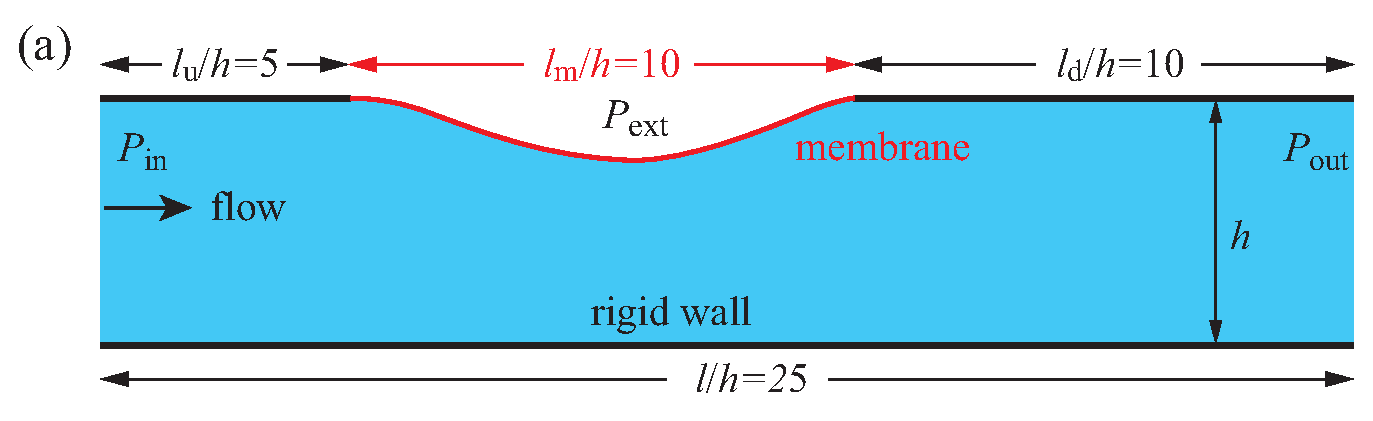
\includegraphics[width=1\linewidth, trim={0cm 0cm -0.35cm
	%0cm}, clip]{./epsFig/fig1a.eps}
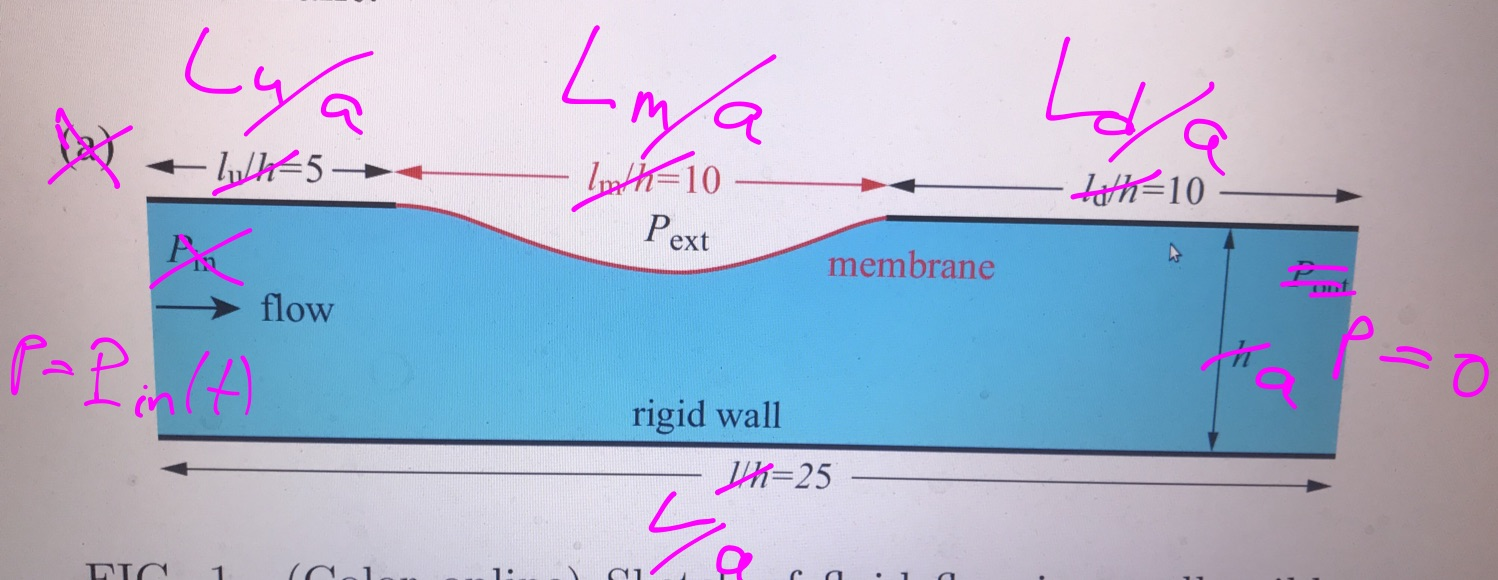
\includegraphics[width=1\linewidth]{matthias_sketches/fig1.jpg}
	\caption{\label{fig:setup}(Color online) Sketch of fluid
          flow in a collapsible channel with an externally pressurized
          membrane clamped between two rigid walls. The flow is driven
          by a pulsatile pressure applied at the upstream end.}
\end{figure}

In this \emph{Letter}, we study the dynamics of pulsatile,
pressure-driven flow in a collapsible channel. We show that the
system exhibits strong resonances, reminiscent of a
forced damped harmonic oscillator. Guided by this observation, we develop
a simple mathematical model which successfully predicts the
oscillation amplitude, the phase lag between the
amplitude and the imposed pressure and also the vanishing of resonances
as the damping is increased {\bf *** Check that the latter is still true***}.

Fig. \ref{fig:setup} shows the problem setup.
A pulsatile pressure with mean $P_0$ and frequency $\Omega$
drives fluid of kinematic viscosity $\nu$ and density $\rho$
through a two-dimensional channel of total length $L$ and height $a$.
The lower channel wall is rigid, whereas a pre-stressed, elastic
membrane of length $L_\text{m}$ is clamped
between two rigid segments at the upper wall and is pressurized by an external
pressure $P_\text{ext}$.

The fluid motion is governed by the incompressible Navier--Stokes
equations, which in dimensionless form read
\begin{equation}
\dfrac{\partial {\bf u}}{\partial t} + {\bf u} \cdot \nabla {\bf
u} = -\nabla  p + \nabla^2  {\bf u},\quad
\nabla \cdot {\bf u}= 0.
\label{eq:NSeqn}
\end{equation}
Here and elsewhere all lengths are scaled on the channel height,
$a$, and time on the timescale for viscous diffusion, $a^2/\nu$.
The fluid velocities are non-dimensionalised on $\nu/a$ and the
pressure on $\rho\nu^2/a^2$.
We set the pressure at the downstream end of the channel to zero
and drive the flow by setting the non-dimensional pressure at the
upstream end to
\begin{equation}
\label{inflow_bc}
p = p_{\rm in}(t)=12 \Rey \,l \left(1 + \sin\,(\alpha^2 \, t)\right).
\end{equation}
Here the non-dimensional forcing frequency $\alpha^2 = \Omega a^2/\nu$ is
a Womersley number and thus characterises the ratio of the
timescale for viscous diffusion to the period of the imposed pressure variation.
The Reynolds number $\Rey = a{\cal U}/\nu$ is formed with the the mean
speed of the Poiseuille flow that would be generated by a steady pressure
drop $P_0$ in the undeformed channel, ${\cal U} = P_0 a^2/(12 \rho \nu
L)$. The boundary conditions for the velocity are no-slip on the walls,
while parallel flow is assumed at the inflow and outflow
boundaries. The lengths of the two rigid segments upstream and
downstream of the elastic membrane were chosen long enough not to
influence the emerging flow patterns. 

We model the elastic segment as a thin, massless
membrane (of thickness $\mathfrak{h}$ and Young's modulus $E$, subject to a
pre-stress $\Sigma_0$) which deforms in
response to the combined effects of the external pressure
and the fluid traction. The resulting traction acting on the
membrane, non-dimensionalised on Young's modulus, is given by
\begin{equation}
\label{eq:nondimloadvector}
{\bf f}=-p_\text{ext} {\bf n} + \frac{1}{H} \left[ p {\bf n} -
  \left(\nabla {\bf u} + (\nabla {\bf u})^T\right) \cdot {\bf n} \right].
\end{equation}
Here ${\bf n}$ is the outer normal to the membrane,
$p_\text{ext}=P_\text{ext}/E$ is the dimensionless external
pressure, and  $H=a^2 E/(\rho\nu^2)$  is a non-dimensional parameter
that represents the ratio of the elastic modulus of the membrane to
the fluid pressure scale. 

We parametrise the shape of the membrane by a dimensionless
Lagrangian coordinate $\xi$ so that the position vector
to a material point in the membrane is
given by ${\bf R}(\xi,t) = {\bf r}(\xi) + {\bf d}(\xi,t)$. Here ${\bf
  r}(\xi) = [\xi, 1]^T$ defines the undeformed configuration and $
{\bf d}(\xi,t)$ is the displacement vector. The membrane
deformation is governed by the principle of virtual displacements
\begin{equation}
\label{eq:virtualdisplacement}
\int_{0}^{l_\text{m}} \left((\sigma_0 + \gamma)\delta \gamma
+ \frac{1}{12}h^2\kappa \,\delta\kappa -
\frac{\Lambda}{h} \ {\bf f} \cdot \delta {\bf R} \right) d\xi = 0,
\end{equation}
where $h=\mathfrak{h}/a$ is the dimensionless thickness of the membrane,
$\gamma=\partial d_x/\partial {\xi} + \frac{1}{2}[(\partial d_x/\partial
  {\xi})^2 + (\partial d_y/\partial {\xi})^2]$ the strain tensor, and
$\kappa = [(\partial^2 d_y/\partial {\xi^2})(1+\partial d_x/\partial
  {\xi}) - (\partial^2 d_y/\partial {{\xi}^2}) (\partial d_y/\partial
  {\xi})]/\Lambda$ the bending tensor, with $\Lambda=[(1+\partial
  d_x/\partial \xi)^2+(\partial d_y/\partial {\xi})^2]^{1/2}$.
The pre-stress is non-dimensionalised on Young's modulus, 
$\sigma_0 = \Sigma_0/E$. We solved the time-dependent fully-coupled 
fluid-structure interaction problem with
the open-source library {\tt oomph-lib} \cite{OOmph,heil2006}.
All simulations shown in this study were performed using the
dimensions shown in Fig. \ref{fig:setup}; the non-dimensional 
membrane thickness was kept constant at $h=10^{-2}$.
\begin{figure}
  \centering
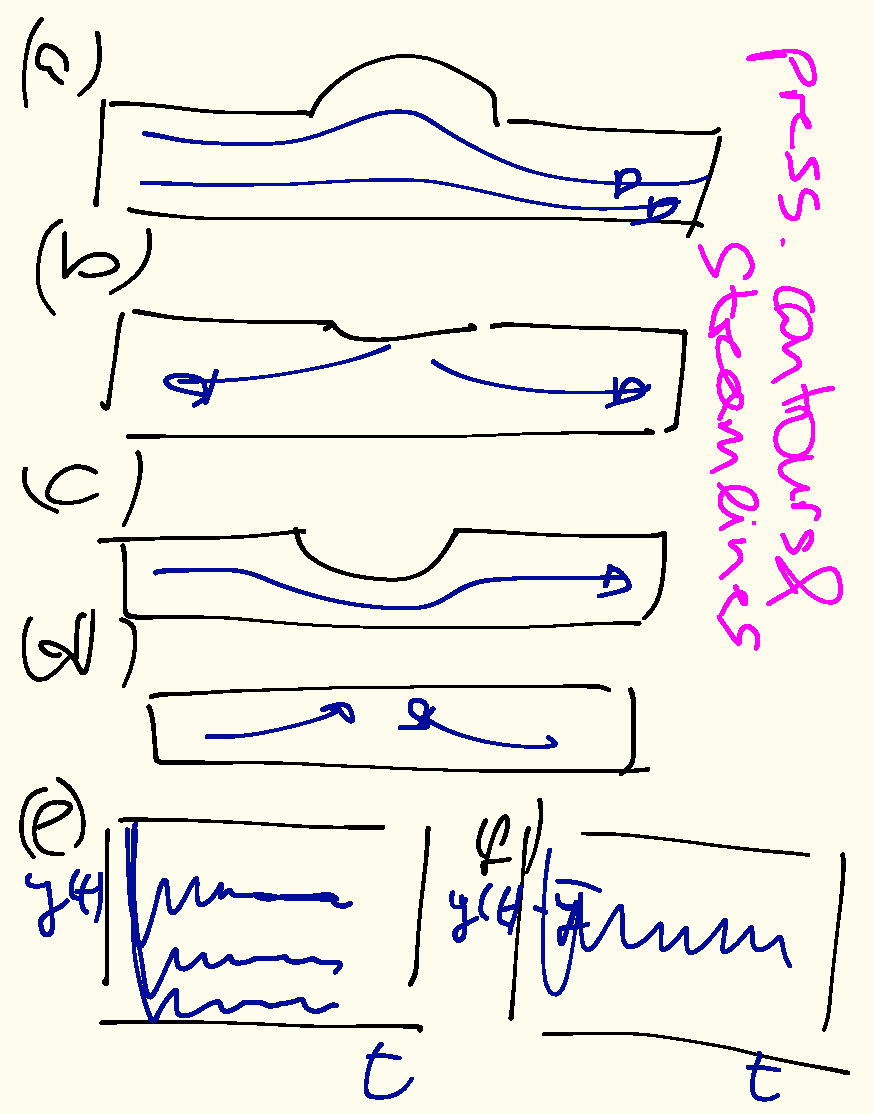
\includegraphics[width=1.0\linewidth]{matthias_sketches/fig2.pdf}
%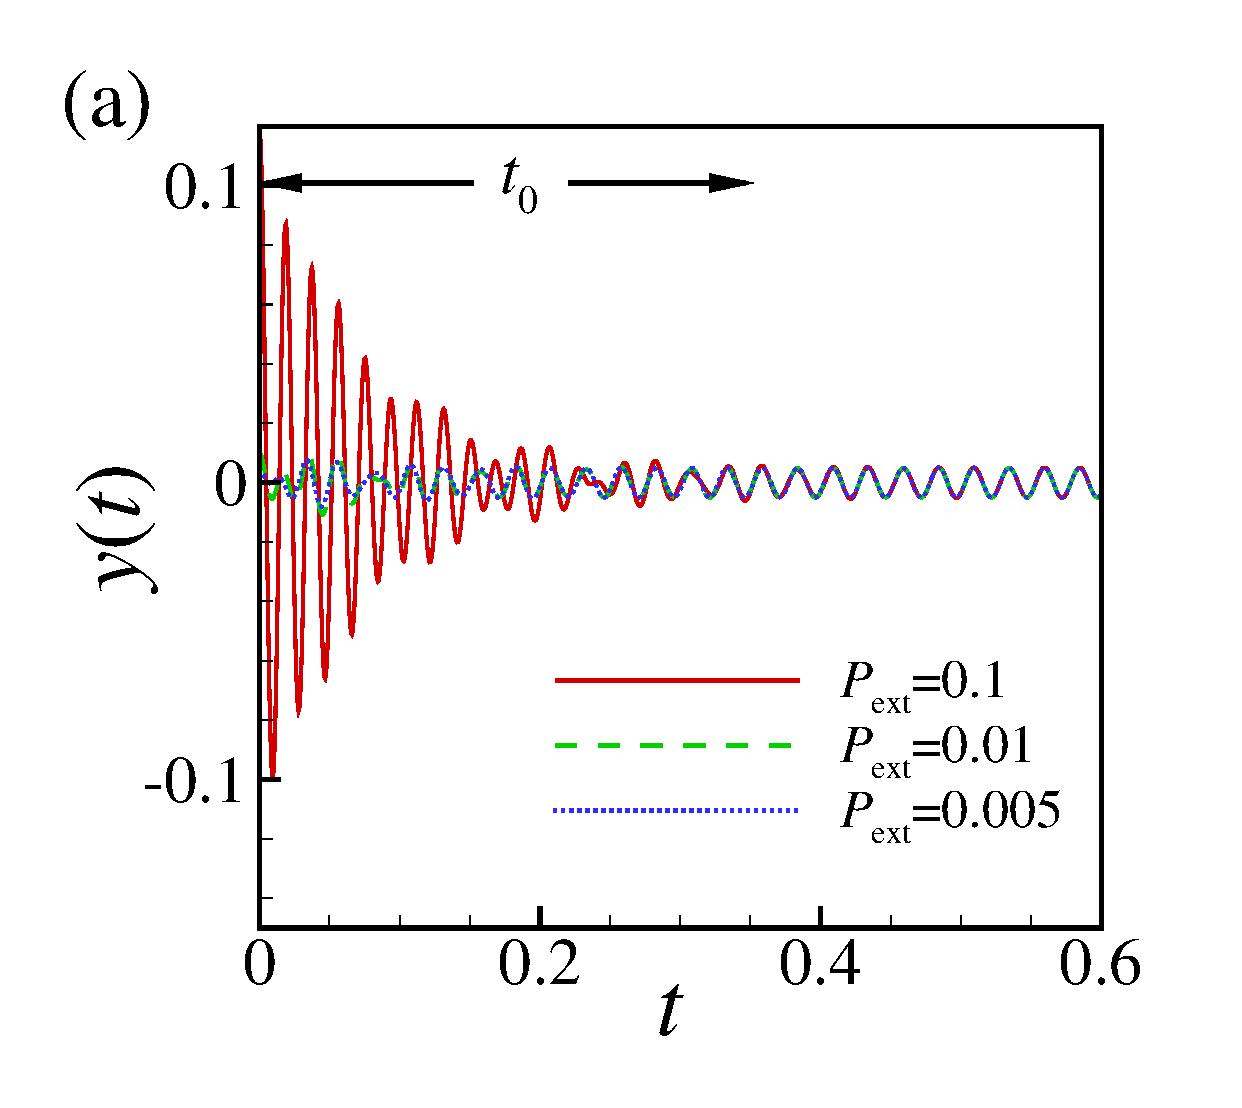
\includegraphics[width=0.49\linewidth, trim={0.5cm 0.5cm 1.5cm 0.5cm}, clip]{./epsFig/fig2a.eps}
%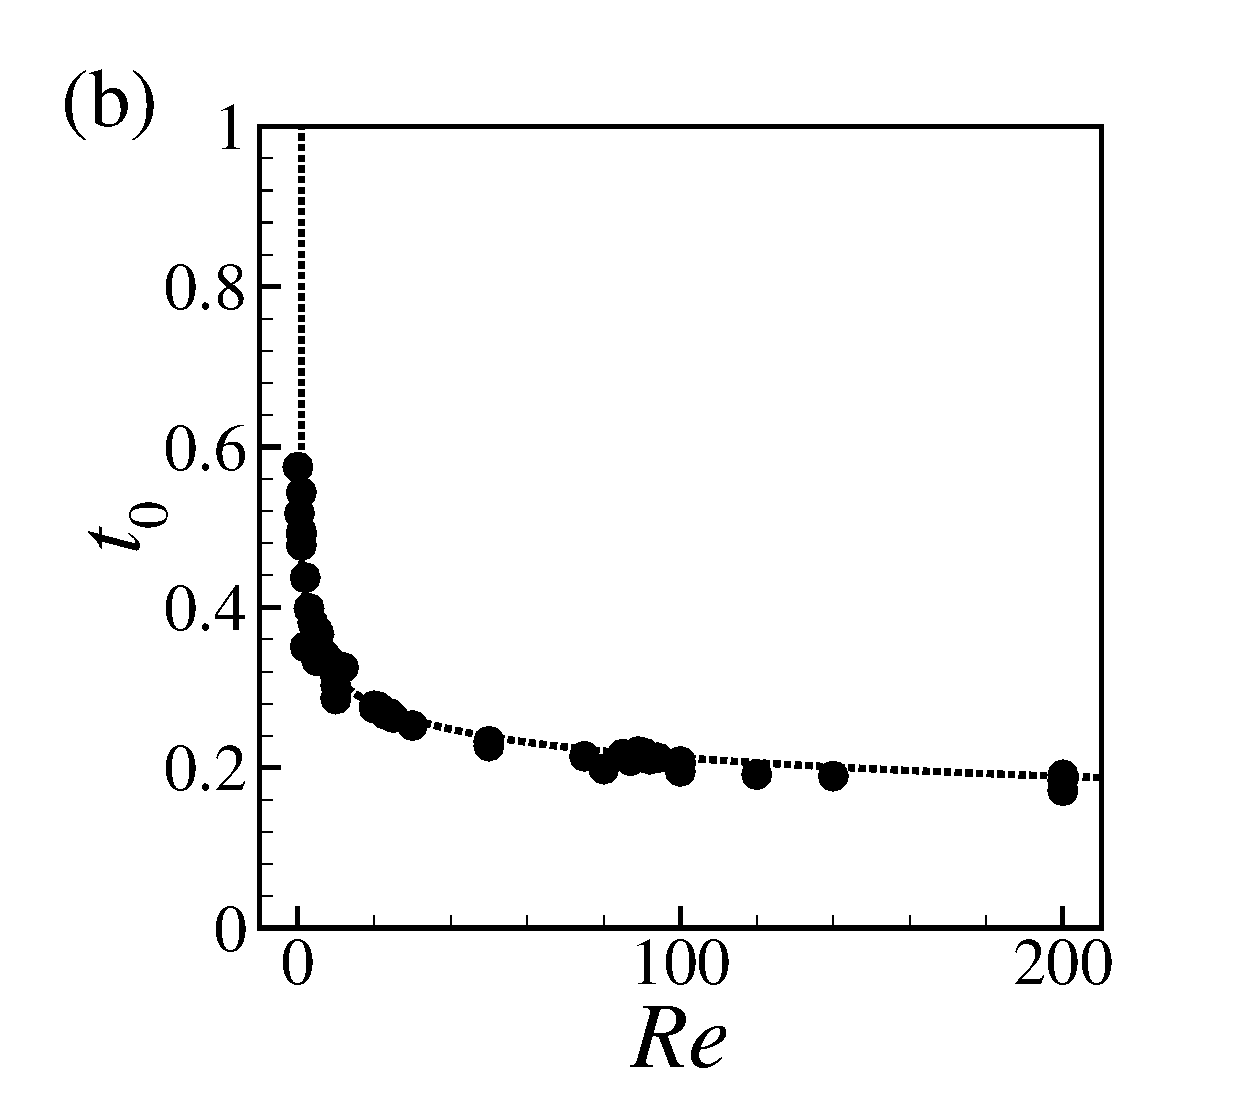
\includegraphics[width=0.49\linewidth, trim={0.5cm 0.5cm 1.5cm 0.5cm}, clip]{./epsFig/fig2b.ep}
  %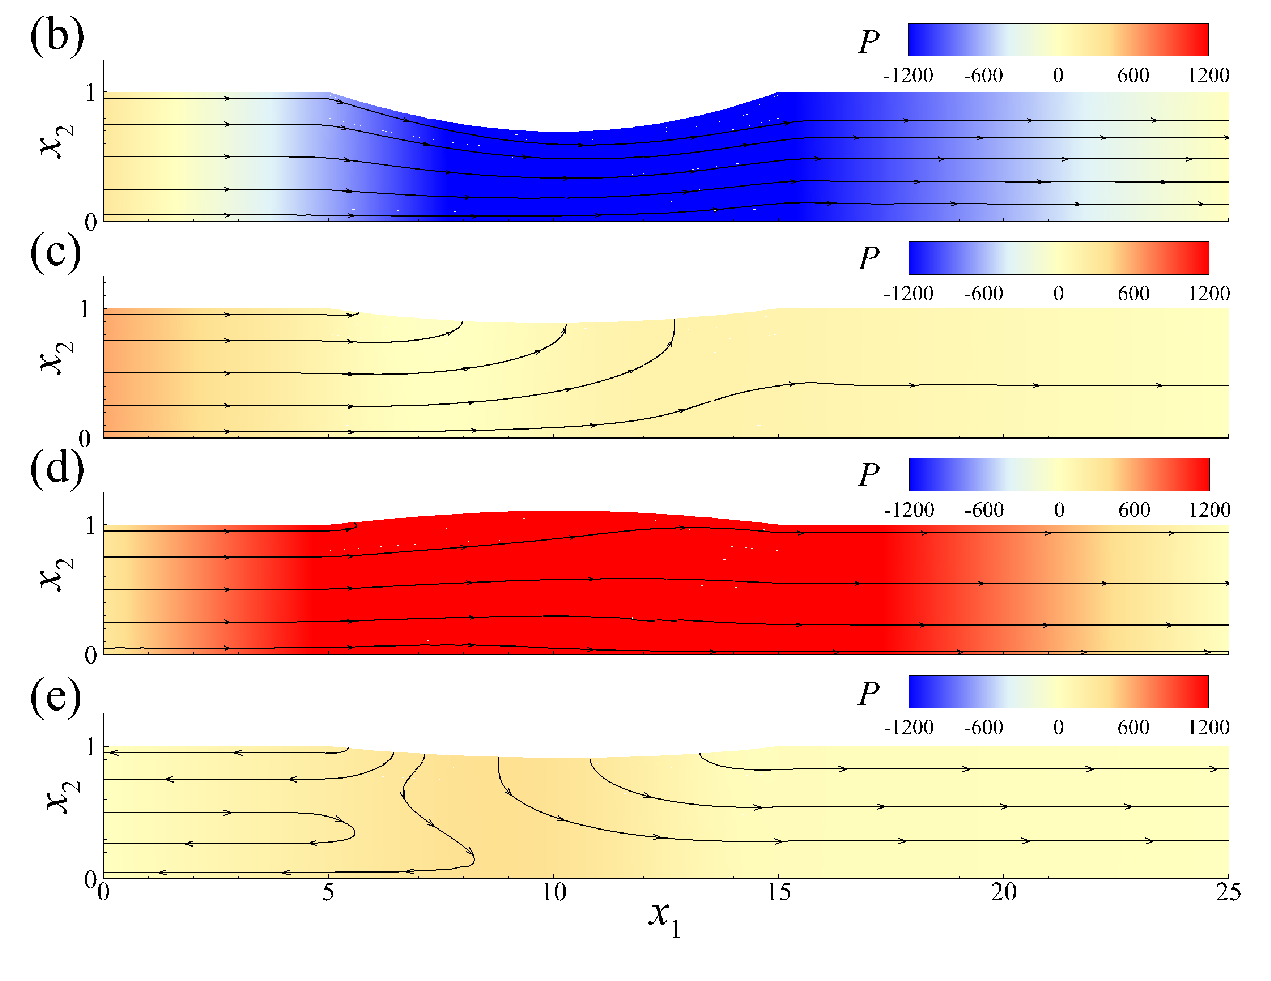
\includegraphics[width=1\linewidth, trim={0.2cm 0cm 0cm 0cm},
  %clip]{./epsFig/fig1b.eps}
%  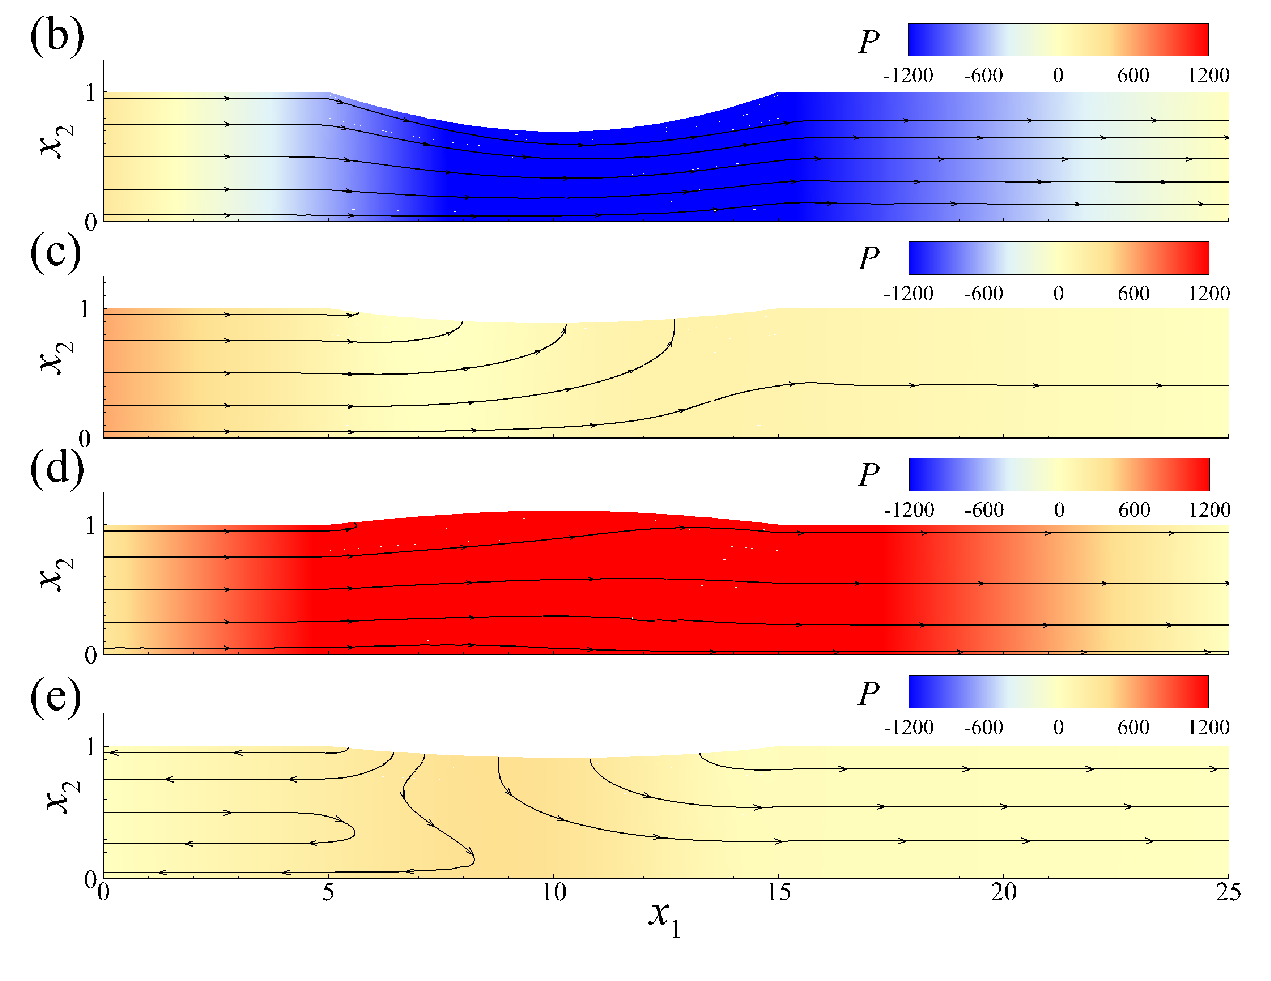
\includegraphics[width=1\linewidth]{./epsFig/fig1b.eps}
\caption{\label{fig:flow_fields_and_displacement}
  (Color online)  (a)-(d) Contour of pressure
  and streamlines at four equally-spaced
  instants throughout the period of the time-periodic oscillation
  following the decay of the initial transients for
  $p_\text{ext}=***$. (e) Time trace of the vertical
  displacement of the membrane mid-point, $y(t)$, for three different 
  external pressures ($p_\text{ext}=***$, $***$
  and $***$). (b) The same data after subtracting the
  time-averaged displacements $\overline{y}$ following the decay of the
  initial transients ($\overline{y} = ***, ***, ***$,
  respectively). $\Rey=***$, $\alpha^2=***$, and
  $H=***$ for all plots.}
\end{figure}
We start the simulations from an initial condition in
which the membrane is undeformed and the velocity
field is steady Poiseuille flow. For a sufficiently large external
pressure the membrane is pushed inwards and, following 
the decay of initial transients the system settles into a
time-periodic (approximately harmonic) motion with the period of the
forcing, $2\pi/\alpha^2$. Figs. \ref{fig:flow_fields_and_displacement}(a-d)
show ... {\bf *** BRIEFLY DISCUSS FLOW FIELDS; POINT OUT THAT IT'S 
LARGE-AMPLITUDE, NONLINEAR, STRONG FSI etc.***}

We characterise the dynamics of the system by monitoring the vertical
displacement {\bf *** CAREFUL ABOUT DISPLACEMENT VS. POSITION ***}
of the membrane at its midpoint, $y(t)$. 
Fig.~\ref{fig:flow_fields_and_displacement}(e) shows time traces of this 
quantity for a range of external pressures. In
Fig.~\ref{fig:flow_fields_and_displacement}(f) we plot
the same data but subtract the time-average displacement
$\overline{y}$ following the decay of the initial transients. This shows
that the amplitude of the time-periodic oscillation, $\widehat{y}$,
is approximately independent of the external pressure (and from now on we set
$p_\text{ext}=0.1$).
{\bf *** DON'T UNDERSTAND THE FOLLOWING SENTENCE ``Note that this
behaviour is in contrast to self-excited oscillations generated by a
constant pressure gradient \cite{Tang15}.'' HOW CAN A CONSTANT
PRESSURE
GRADIENT GENERATED OSCILLATIONS; IF THEY'RE SELF-EXCITED THEN IT'S
A TOTALLY DIFFERENT PROBLEM! DISCUSSED WITH MARC: WHAT'S MEANT IS THAT
ONSET DEPENDS ON PEXT; BIT SUBTLE...***}
The duration of the initial transients is on the order of the
viscous time unit, $\nu/a^2$. This suggests
that the adjustment toward a time-periodic oscillation is 
controlled by the viscosity of the fluid.

\begin{figure}
\centering
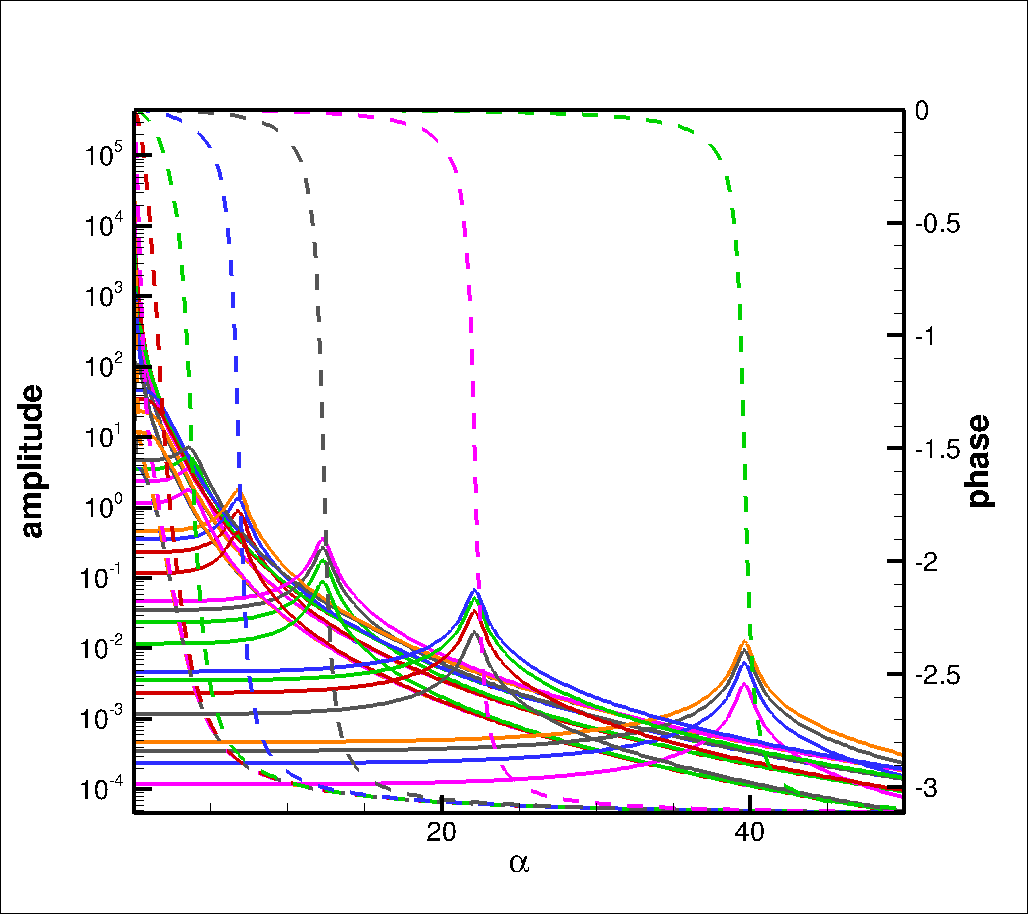
\includegraphics[width=1.0\linewidth]{maple/all_sigma0_times_H.png}	
%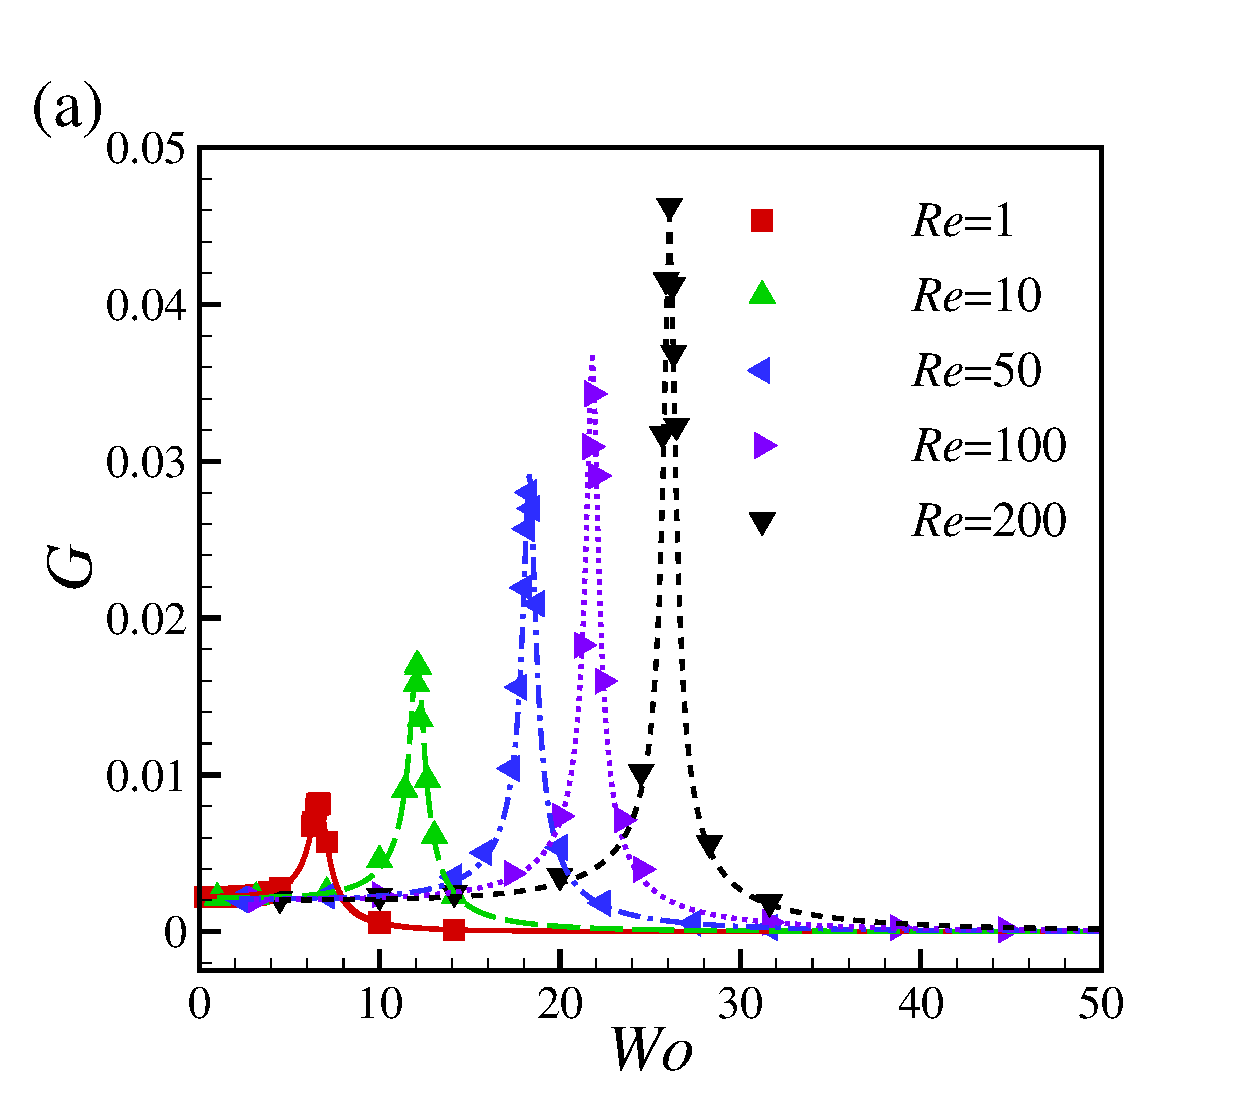
\includegraphics[width=0.49\linewidth, trim={0.3cm 0cm 1.75cm 1cm}, clip]{./epsFig/fig3a.eps}	
%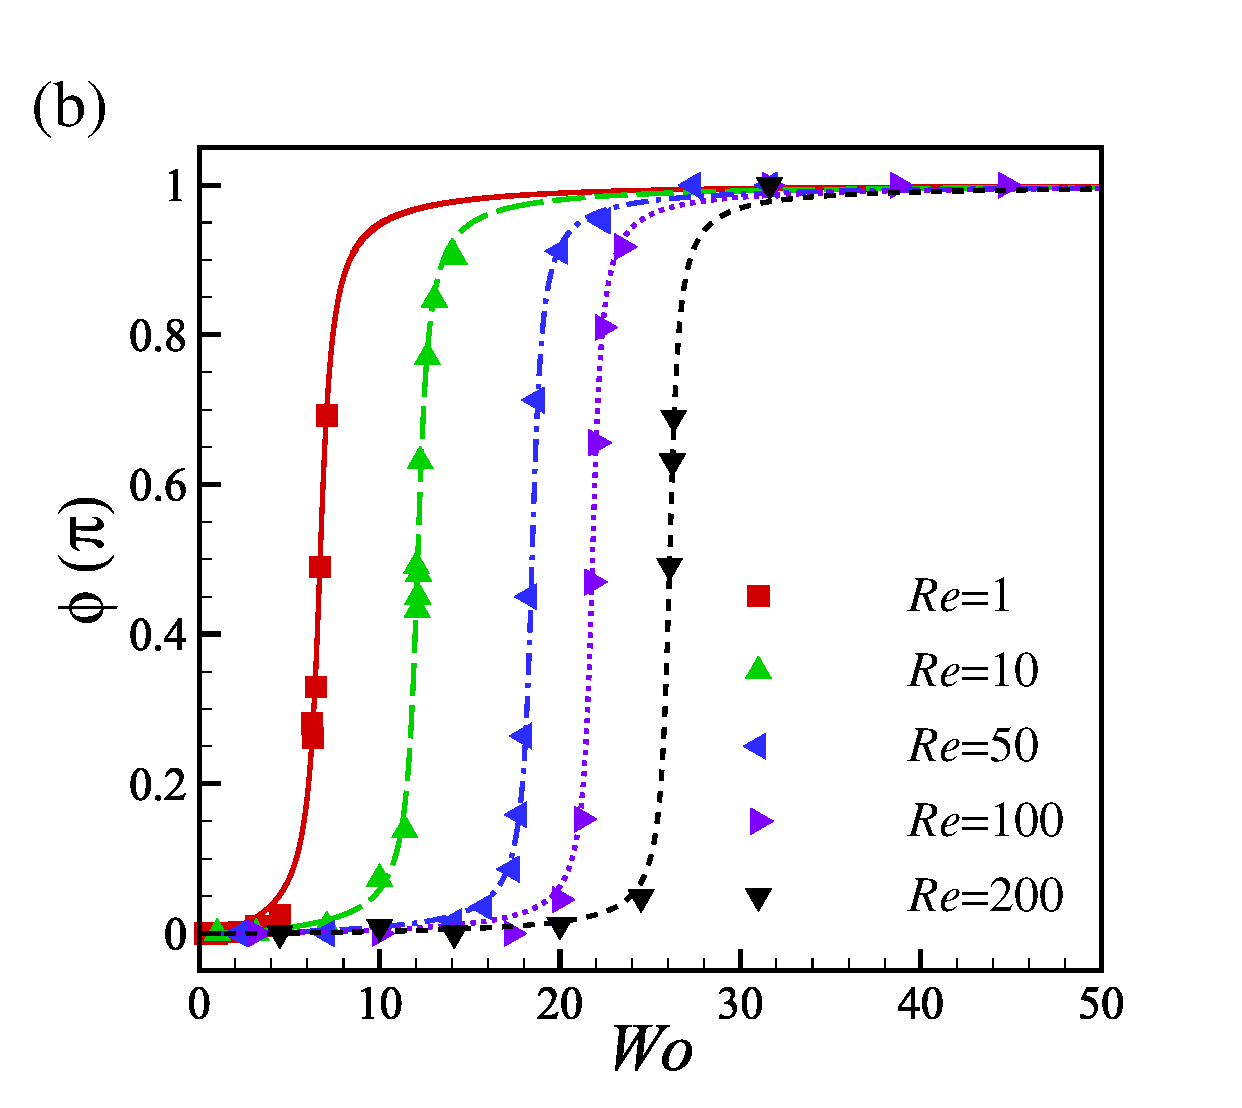
\includegraphics[width=0.49\linewidth, trim={0.3cm 0cm 1.75cm 1cm}, clip]{./epsFig/fig3b.eps}
\caption{\label{fig:amplitude_phase}(Color online) (a) Amplitude and
  (b) phase shift of the steady-state oscillations as a function of
  the dimensionless frequency parameter $\alpha$ {\bf ***$\alpha^2$ is
  probably better as it represents the frequency***} for several
  values of the Reynolds number $Re$ and $H$.
  Here $p_\text{ext}=0.1$ and $\sigma_0=***$.
  {\bf ** Split into (a) and (b) and use the real (oomph-lib!) data **}
}
\end{figure}

We now focus on the dynamics of the steady-state oscillations following
the decay of the transients. Fig.~\ref{fig:amplitude_phase}(a) shows the
amplitude of the oscillations, $\widehat{y}$, against the
non-dimensional forcing frequency $\alpha^2$ for different values of the
parameters $Re$ and $H$ while keeping the pre-stress $\sigma_0$ constant.
The amplitude of the membrane oscillation has a sharp maximum at
$\alpha^2 \approx ***$, which appears to be independent of the 
Reynolds number. Furthermore, the phase $\phi$ between the forcing 
pressure, $P(t)$, and $y(t)$ varies displays a $180^{o}$ phase shift 
when the amplitude reaches is maximum.

This behaviour is reminiscent of the response of the forced damped
harmonic oscillator...


\hrule


\newpage


\section{APPENDIX (?) Derivation of the linear oscillator model}
We will now develop a simple model that describes the response
of the collapsible channel to the imposed pressure fluctuations at
its upstream end. Since we found the external pressure to have
little effect on the system's behaviour, we set it to
zero and thus consider the setup shown in Fig. \ref{model.png}(a).
\begin{figure}
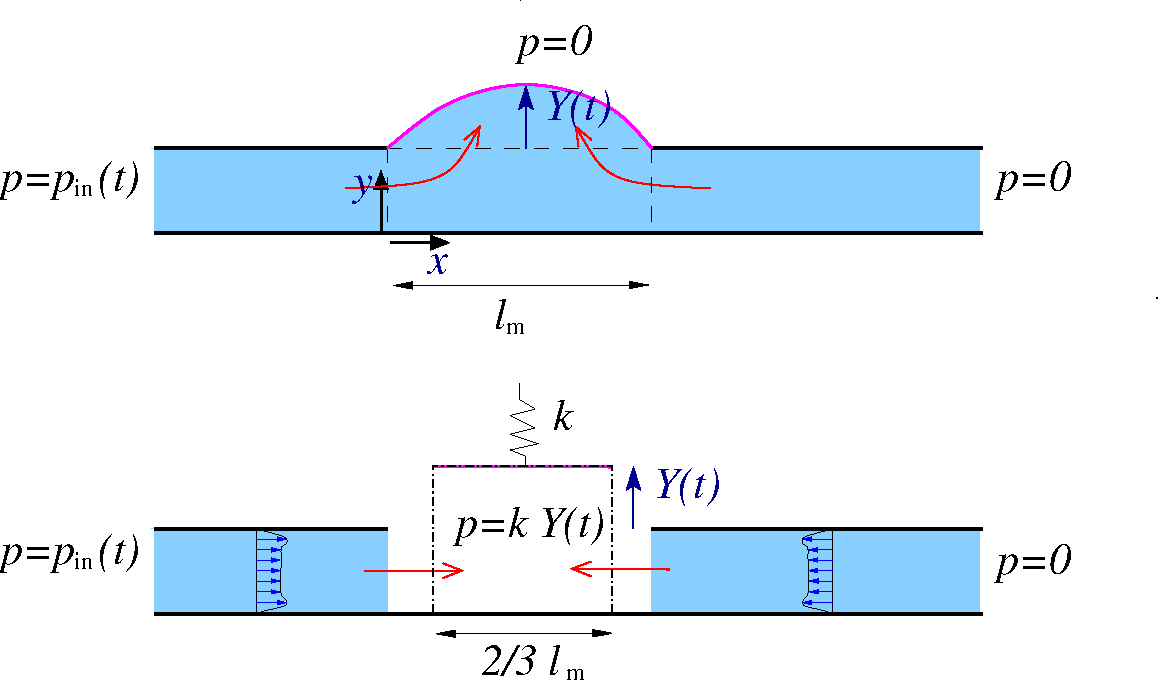
\includegraphics[width=0.99\linewidth]{pictures/model.png}
\caption{\label{model.png}bla}
\end{figure}
  We assume the upstream and downstream rigid parts of
the channel to be sufficiently long, $l_{\rm u}, l_{\rm d} \gg 1$, so that the 
horizontal component of the velocity, $u$, is much larger
than its vertical counterpart. Our computations
show that this assumption is appropriate even in the relatively
short channels used in our simulations. The horizontal component of
the momentum equation (\ref{eq:NSeqn}) can then be approximated by 
\be
\label{long_wavelength_momentum}
\frac{\partial u}{\partial t} = -\frac{\partial p}{\partial x} +
\frac{\partial^2 u}{\partial y^2},
\ee
where the pressure gradient only depends on time, 
$\partial p/\partial x = G(t)$, and we have $u=u(y,t)$. We assume that the
vertical displacement of the elastic membrane can be described by the
product of a mode shape $M(x)$ and an amplitude $Y(t)$, so that
\be
y_m(x,t) = 1+ Y(t) M(x).
\ee
Based on the shapes observed in the computations,
we approximate $M(x)$ by a quadratic function,
$M(x) = 4 (x/l_{\rm  m})(1-(x/l_{\rm m}))$. Given that the 
elastic membrane is under a large, approximately constant tension we describe
its deformation by Laplace's law, implying that the fluid pressure
in the elastic segment is given by the product
of the membrane curvature and its tension. For the assumed mode shape
the non-dimensional fluid pressure under the membrane is then given by
\be
\label{p_m}
p_{\rm m} = k Y(t),
\ee
where the dimensionless constant $k$ is
\be
k = \frac{8 h \sigma_0 H}{l_{\rm m}^2}
= \frac{\Sigma_0 \mathfrak{h}a^3}{\rho \nu^2 L_{\rm m}^2}.
\ee
Since the pressure gradient in the upstream and downstream rigid
segments is spatially constant, the momentum equation
(\ref{long_wavelength_momentum}) becomes
\be
\label{upstream_mom}
\frac{\partial u_{\rm u}(y,t)}{\partial t} =
-\frac{k Y(t) - p_{\rm in}(t)}{l_{\rm u}} +
\frac{\partial^2 u_{\rm u}(y,t)}{\partial y^2}
\ee
and
\be
\label{downstream_mom}
\frac{\partial u_{\rm d}(y,t)}{\partial t} =
\frac{k Y(t)}{l_{\rm d}} +
\frac{\partial^2 u_{\rm d}(y,t)}{\partial y^2},
\ee
respectively.
The flows in the two rigid segments are coupled by
mass conservation which requires that the
rate of change in the volume of the elastic segment
\be
\int_0^{l_{\rm m}} \frac{\partial y_{\rm m}}{\partial t} \ {\rm d}x =
\frac{{\rm d}Y}{{\rm d}t} \int_0^{l_{\rm m}} M(x) \ {\rm d}x  = 
\frac{2}{3} \ l_{\rm m} \ \frac{{\rm d}Y}{{\rm d}t}.
\ee
is matched by the net volume flux from the rigid segments, so that
\be
\label{conti}
\frac{2}{3} \ l_{\rm m}  \ \frac{{\rm d}Y}{{\rm d}t}
= \int_0^1  (u_{\rm u} - u_{\rm d} ) \ {\rm d}y.
\ee
Equations (\ref{p_m}), (\ref{upstream_mom}), (\ref{downstream_mom})
and (\ref{conti}) imply that the collapsible
channel behaves like the linear oscillator sketched in 
Fig. \ref{***}(b): The elastic membrane of length $l_{\rm m}$
is equivalent to a piston of width $\frac{2}{3}l_{\rm m}$, mounted on a spring
of stiffness $k$. The piston is displaced by the net influx of
fluid from the rigid segments and sets the fluid pressure acting at
their internal boundaries. The system's oscillations are
governed by a dynamic balance between fluid inertia and the
elastic restoring forces, with the fluid viscosity providing
damping.

To explore under what conditions the system displays resonant
behaviour we consider the case of a purely oscillatory forcing, $p_{\rm in}(t) =
\widehat{P} \exp({\rm i}\alpha^2 t)$ and assume a time-periodic response such
that $Y(t) = \widehat{Y} \exp({\rm i}\alpha^2 t)$ and
$u_{\rm u/d}(y,t) = \widehat{U}_{\rm u/d}(y) \exp({\rm i}\alpha^2
t)$. Inserting this ansatz into (\ref{upstream_mom}) and
(\ref{downstream_mom}) and solving the resulting ODEs, subject to
the no-slip boundary conditions $\widehat{U}_{\rm u/d}(y=0,1)=0$,
we obtain $\widehat{U}_{\rm u/d}(y)$ in terms
of $\widehat{Y}$ and $\widehat{P}$.
Inserting $\widehat{U}_{\rm u/d}(y)$ into (\ref{conti}) then
establishes a relation between $\widehat{P}$ and $\widehat{Y}$. Since the
amplitude of the imposed oscillatory pressure fluctuation is related
to the Reynolds number and the non-dimensional total channel length
via $\widehat{P} = 12 l \Rey$ (cf. equation (\ref{inflow_bc})), we obtain
the (complex) amplitude $\widehat{Y}$ of the membrane oscillation
as a function of the channel geometry ($l_{\rm u}, l_{\rm m}, l_{\rm
  d}$) and the non-dimensional parameters $k$, $Re$ and $\alpha^2$.
The algebra involved in these calculations is straightforward but
lengthy and was performed with {\tt maple}. The results are
shown by the ***ed lines in Fig. \ref{****} which show ****.
{\bf *** MENTION THAT AMPLITUDE IS $|\widehat{Y}|$ AND PHASE
  ANGLE IS ITS ARGUMENT. ***}

 Additional insight can be gained by differentiating (\ref{conti})
with respect to time and inserting $\partial u_{\rm u/d}/\partial t$
from (\ref{upstream_mom}) and (\ref{downstream_mom}) which yields
\be
\frac{2}{3}l_{\rm m} \frac{{\rm d}^2 Y}{{\rm d}t^2} +
k \frac{l_{\rm u} + l_{\rm d}}{l_{\rm u} l_{\rm d}} \ Y
+ \left.
\left( \frac{\partial u_{\rm d}}{\partial y} -
       \frac{\partial u_{\rm u}}{\partial y} \right)
\right|_{y=0}^1 = \frac{p_{\rm in}(t)}{l_{\rm u}}.
\ee
The last term on the left hand side of this equation arises from the
viscous terms in the momentum equation and represents the effect of
the viscous shear stresses acting on the walls of the rigid segments.
The remaining terms show that in the absence of viscous damping
the system is a forced linear oscillator with eigenfrequency
\be
\alpha_{\rm eig}^2 = \left( 
\frac{3}{2} \frac{k}{l_{\rm m}}
\frac{l_{\rm u} + l_{\rm d}}{l_{\rm u} l_{\rm d}}.
\right)^{1/2}
\ee
While this basic model yields good qualitative agreement
with the computational results, Fig. \ref{***} shows that
it over-estimates the eigenfrequency. This is a consequence of us
having neglected the dynamics of the fluid that moves within the
elastic segment itself. We can include this effect heuristically by replacing
$l_{\rm u/d}$ by corresponding effective lengths $l_{\rm u/d}^{\rm [eff]} =
l_{\rm u/d} + \beta l_{\rm m}$ where the parameter $\beta$
represents the fraction of the fluid in the elastic
segment that participates in the oscillatory motion.


{\bf *** Setting $\beta =  1/4$ works nicely (for our geometry)
and gives perfect agreement with Oliver's theoretical predictions for
the eigenfrequency.
  Found this by trial and error. Can we make this the fitting
  parameter? ***}

\begin{figure}
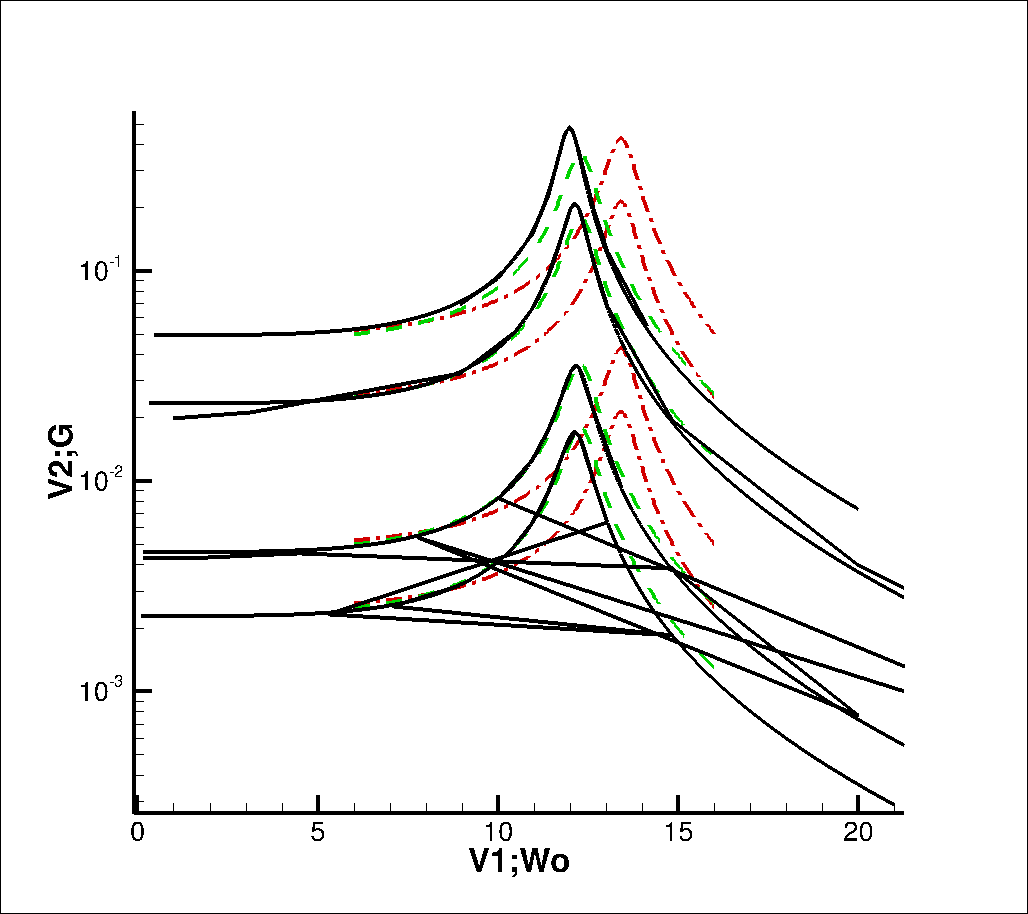
\includegraphics[width=0.99\linewidth]{maple/ampl_comparison.png}
\caption{\label{comparison.png}Black solid: oomph-lib; red dash-dot:
  basic model; green dashed: tweaked model with $\beta = 1/4$.}
\end{figure}


{\bf *** We can make this look even better by plotting for a range of
$H$ values; in fact, vary both $\sigma_0$ and $H$ and show that,
as the theory (and common sense) predict, it's only the product
of the two that matters! ***}

\newpage



in classical mechanics \cite{Shabana91}, which consists of a mass $\widetilde{m}$ attached to a spring with stiffness coefficient $\widetilde{k}$ subject to an external harmonic force of amplitude $\widetilde f$ and frequency $\omega$. In addition, the motion of the mass is damped by viscous force with damping coefficient $c$. The governing equation of the harmonic oscillator is
\begin{equation}
\widetilde m\frac{\partial^2 \widetilde y}{\partial {\widetilde t}^2}=-c\frac{\partial \widetilde y}{\partial \widetilde t}-\widetilde k\,\widetilde y+\widetilde f\sin  \omega \widetilde t,
\label{eq:oscillator_eqn}
\end{equation}	
where $\widetilde y$ is the instantaneous displacement of the mass with respect to the equilibrium position. In what follows, we explore an analogy between the collapsible channel driven by a pulsatile pressure difference and the driven harmonic oscillator. In this analogy, the displacement of the membrane's midpoint $y(t)$ is assumed to exhibit dynamics similar to the spring displacement $\widetilde y(t)$ in the harmonic oscillator. 

In our model, the spring constant $k$ is assumed proportional to the effective Young modulus of the membrane and to its length, i.e.~$\tilde k=A_\text{k}\, E_\text{eff}\,l_\text{m}$, whereas the mass is assumed proportional to the mass of fluid beneath the membrane $\tilde m=A_\text{m}\, \rho\, l_\text{m}\, h^2$. The main driving force is expected to be proportional to the pressure force acting on the membrane $\tilde f=A_\text{f}\,\rho\nu\, \bar{u}\, l_\text{m}$. Note that because the flow is laminar, we choose the viscous scale $\rho\nu\, \bar{u}/h$ for the pressure. The scaling of the viscous damping coefficient $c$ is unclear a priori, so this is left as unknown for the time being. 

Plugging in the expressions for $\tilde m$,  $\tilde f$ and $\tilde k$ above into \eqref{eq:oscillator_eqn} and rendering the equation dimensionless by rescaling lengths with $h$, velocities with $\bar{u}$ and time with $h^2/\nu$, we obtain the following model 
\begin{equation}
\frac{\partial^2 y}{\partial t^2}+C_\text{d}\frac{\partial y}{\partial t}+\left(\Wo^4_0\right)y={\alpha_f}{\Rey}\;\sin\left(\Wo^2 \, t\right),
\label{eq:channel_eqn}
\end{equation}
with $\alpha_f=A_\text{f}/A_\text{m}$ and the drag coefficient $C_\text{d}=c/(A_\text{m}\,\rho\nu\,l_\text{m})$. The model predicts that the eigenfrequency $\Wo_0$ of the collapsible channel depends on the material properties of the fluid-structure interaction as
\begin{equation}\label{eq:model_St0}
\Wo_0=({\alpha_k}H)^{1/4},
\end{equation}
with the constant $\alpha_k=A_\text{k}/A_\text{m}$. The accuracy of the assumptions in our model can be assessed by fitting the simulation data with the well-known analytic steady-state solution of \eqref{eq:channel_eqn} 
\begin{equation}
y(t)=G \text{sin}\left(\Wo^2  t-\phi\right),
\label{eq:channel_solution}
\end{equation}
where 
\begin{equation}
G = \dfrac{{\alpha_f}{\Rey}}{\sqrt{\left(\Wo^4_0-\Wo^4\right)^2+C_\text{d}^2\,\Wo^4}},
\label{eq:channel_gain}
\end{equation}
is the amplitude of the oscillations (typically referred to as gain) and 
\begin{equation}
\phi=\tan^{-1}\left[\dfrac{C_\text{d}\, \Wo^2}{\Wo_0^4-\Wo^4}\right]
\label{eq:channel_phase}
\end{equation}
is the phase delay between driving force and response. In summary, there are three fit parameters, of which two ($\alpha_k$ and $\alpha_f$) should be constant according to the model, whereas the drag coefficient $C_\text{d}$ is expected to depend on the flow parameters and particularly on the Reynolds number. 

\begin{figure}
	\centering
	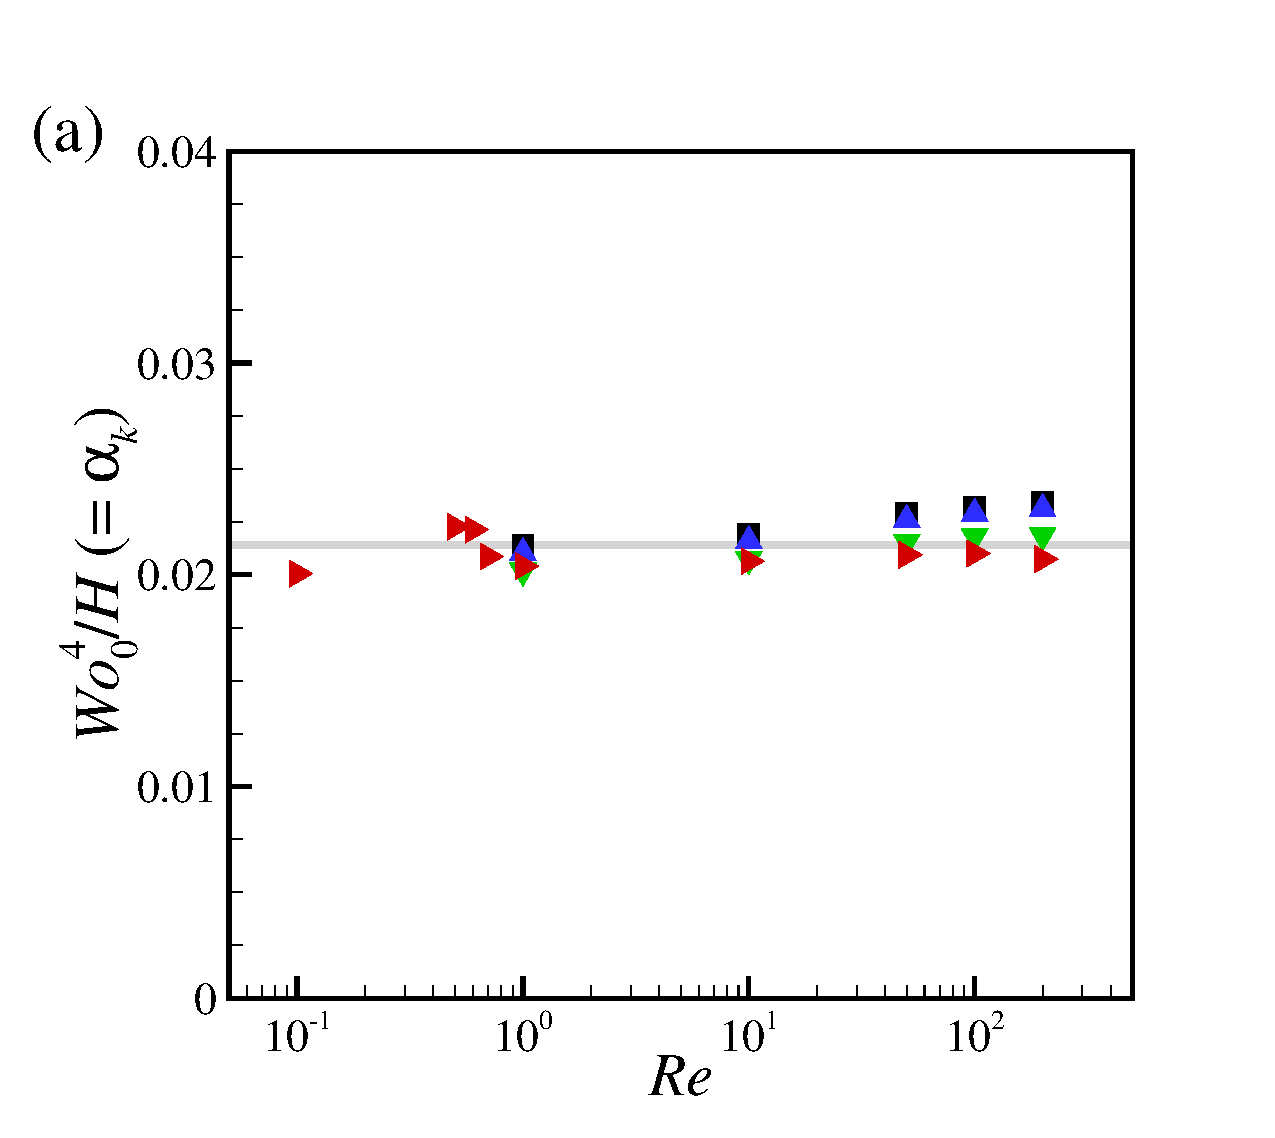
\includegraphics[width=0.49\linewidth, trim={0.25cm 0cm 1.5cm 1.5cm}, clip]{./epsFig/fig4a.eps}
	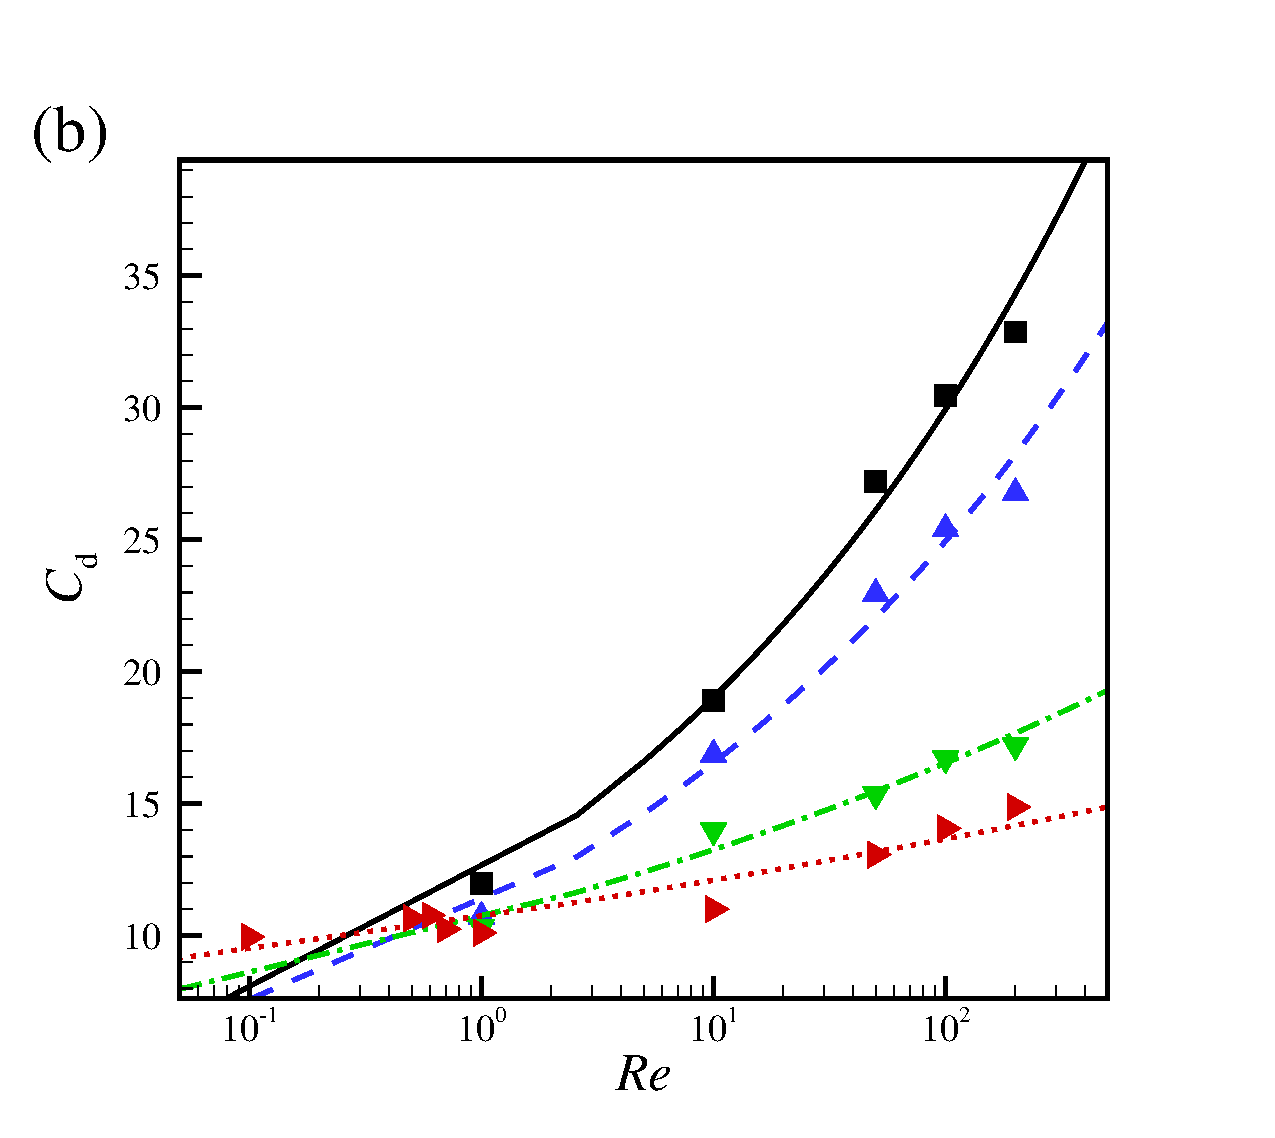
\includegraphics[width=0.49\linewidth, trim={0.25cm 0cm 1.5cm 1.5cm}, clip]{./epsFig/fig4b.eps}
	\caption{\label{fig:Wo0}(Color online) (a) Dimensionless eigenfrequency $\Wo_0$ of the collapsible channel against $\Rey$ for $Q=10^{-5}$ (black squares and black circles), $Q=2 \times 10^{-5}$ (blue up-triangles), $Q=10^{-4}$ (green down-triangles) and $Q=2\times10^{-4}$ (red right-triangles). The gray solid-line shows $\alpha_k=0.02$.	 
	% When I look at the figure is seems to me like the value of \alpha_k should be more like 0.025. How as this obtained?	
	(b) The drag coefficients $C_\text{d}$ varying with $Re$ where the symbols, the same as Fig.~\ref{fig:Str_Rer_Q}, lines are from power law fitting.
	%denote simulation results and the lines are $C_\text{d}=48\Rey(5\Rey)^{g(Q)}$, with $g(Q)=-1.475Q^{0.0495}$ (see Fig X in the supplementary materials). 
	% This figure needs to be redone with a more reasonable y axis. 
	}
\end{figure}


The lines in Fig.~\ref{fig:amplitude_phase}a show the best fits of the gain \eqref{eq:channel_gain} to the oscillation amplitude obtained from the numerical simulations. Indeed, we find that $\alpha_f\approx4.2$ and $\alpha_k\approx0.02$ % Are you sure that you are using this value? When I look into figure 4a, to me it seems more that the value should be 0.025 (it should agree well with the black data points). % Duo: the mean of alpha_k over four sets is 0.0215.
are constants adjusting all data sets, whereas $C_\text{d}$ depends on $\Rey$. The fitted values of $\alpha_f$, $\alpha_k$ and $C_\text{d}$ also render excellent approximations of the phase delay (see lines in Fig.~\ref{fig:amplitude_phase}b). Together these results suggest that the dynamics of the pulsatile collapsible channel can be accurately modeled with a harmonic oscillator. Despite the wide ranges of $\Wo$ and $\Rey$ covered in Fig.~\ref{fig:amplitude_phase}, all these simulations were obtained for $Q=10^{-5}$. This raises the question of whether the model captures the dependency on $Q$ as well, which was investigated here by performing additional sets of simulations for $Q=2\times 10^{-5}$, $10^{-4}$ and  $2\times 10^{-4}$.  Of particular interest is the eigenfrequency prediction (see \ref{eq:model_St0} and recall that $H=Re/Q$). Figure~{fig:Wo0}a confirms our prediction and shows that the eigenfrequency of the collapsible channel depends only on material parameters at low Reynolds numbers $\Rey\le 10$, whereas at higher $\Rey$ small but noticeable differences among the data sets for different $Q$ are observed. On the other hand, the data reveal a complex dependence of the friction coefficient on $\Rey$ and $Q$. In particular, $C_\text{d}$ follows a power-law of the Reynolds number, in which both pre-factor and exponent depend on $Q$ (see Fig.~\ref{fig:Wo0}b). 

\begin{figure}
	\centering	
	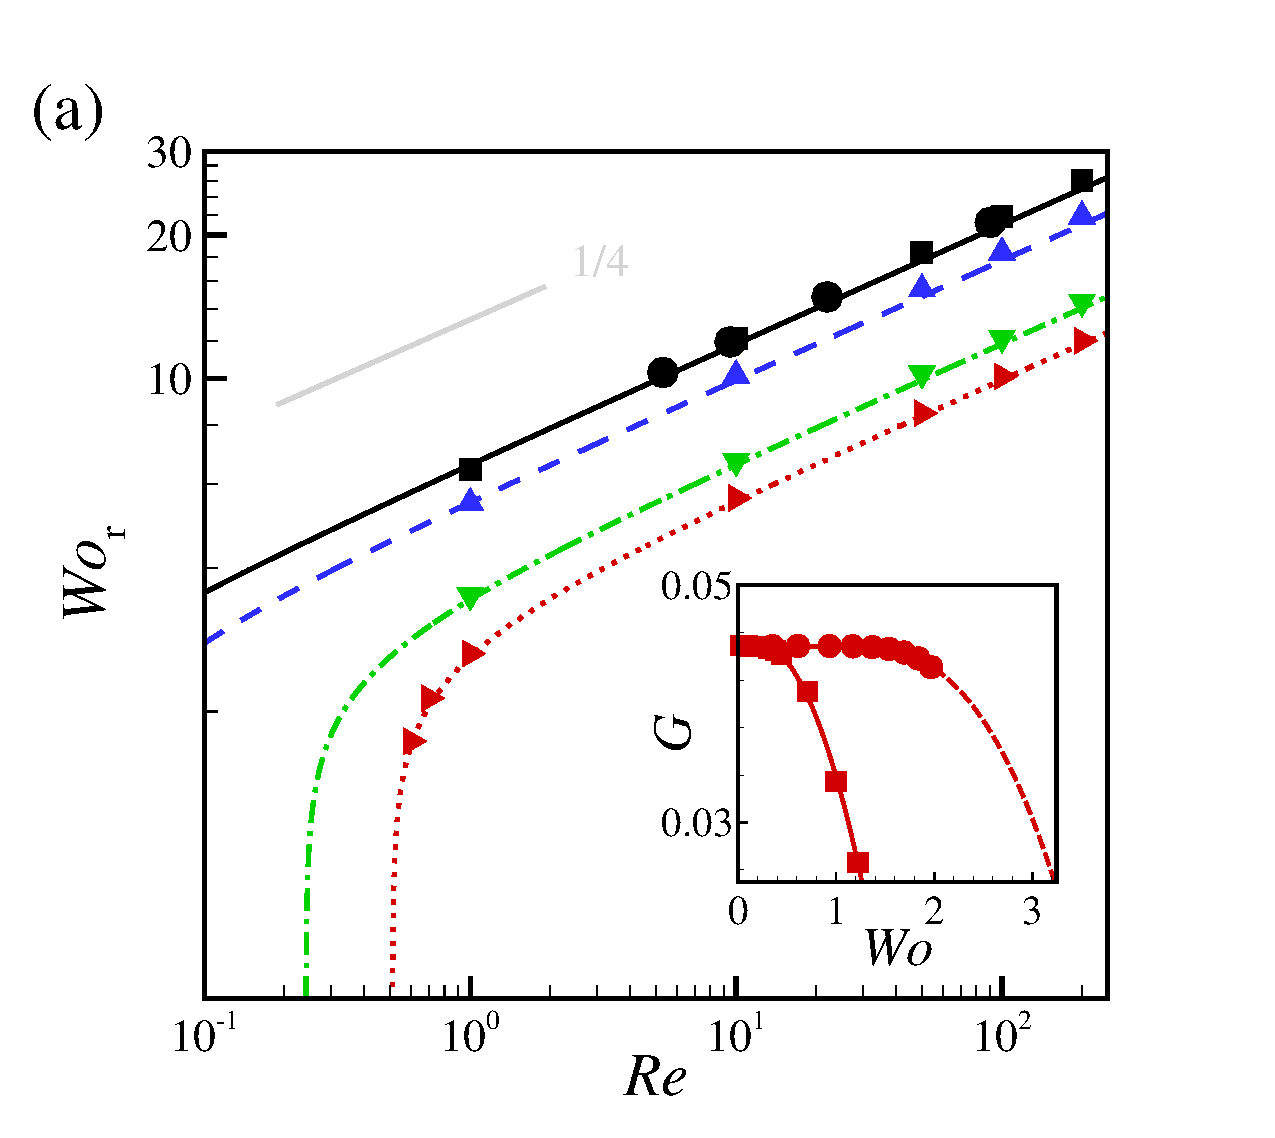
\includegraphics[width=0.49\linewidth, trim={0.25cm 0cm 1.5cm 1cm}, clip]{./epsFig/fig5_sub_a.eps}
	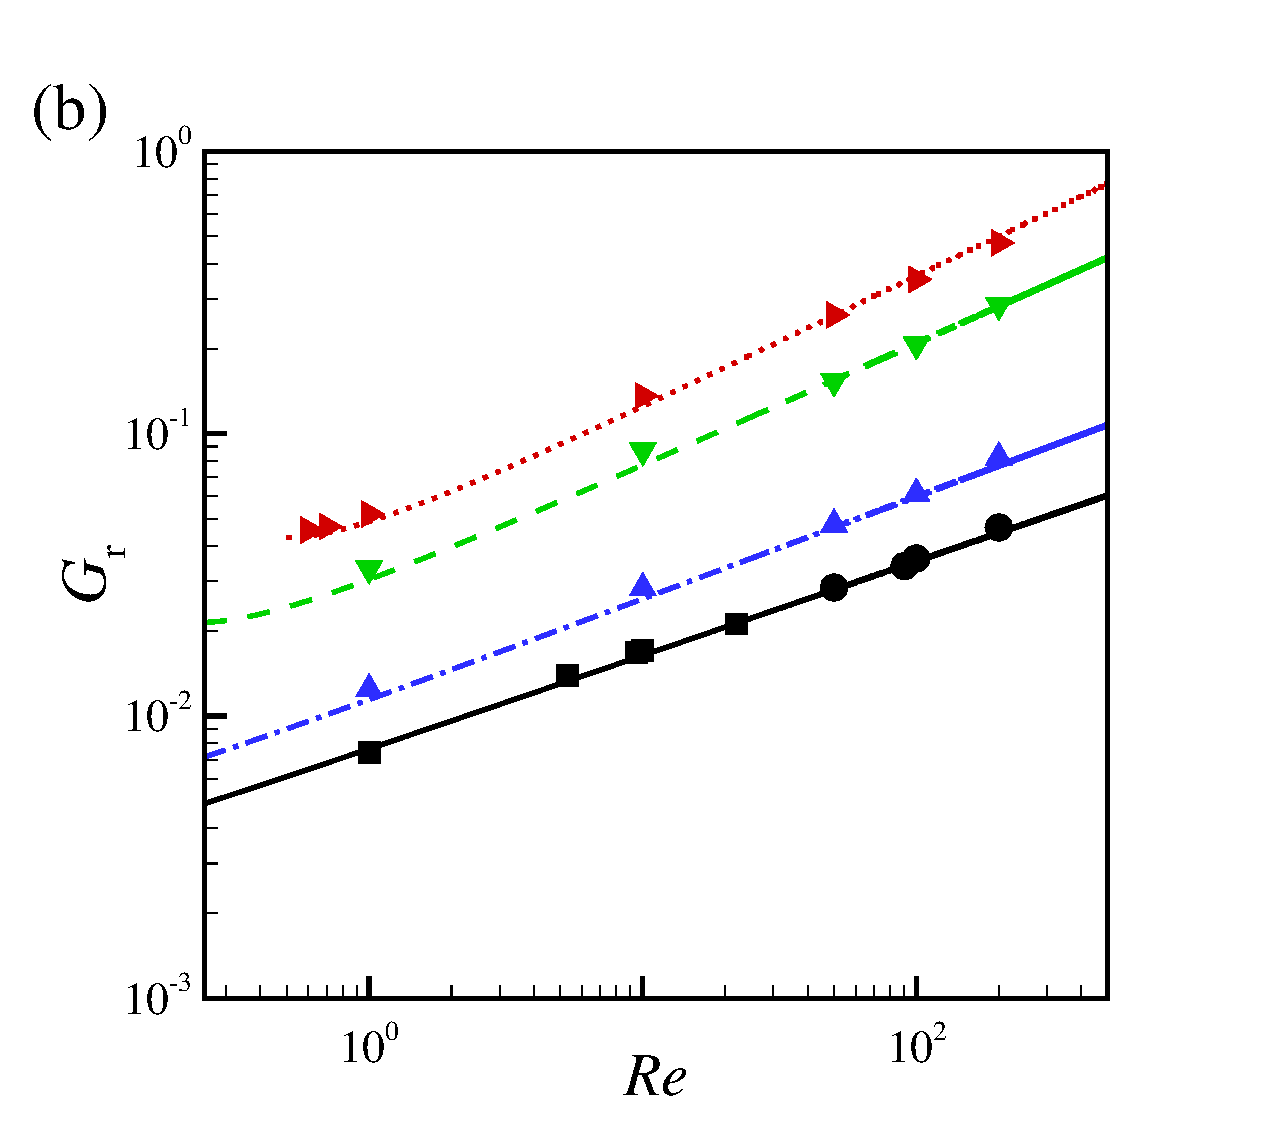
\includegraphics[width=0.49\linewidth, trim={0.25cm 0cm 1.5cm 1cm}, clip]{./epsFig/fig5b.eps}
	\caption{\label{fig:Str_Rer_Q} (Color online)  (a) Resonant points for $Q=10^{-5}$ (black squares and black circles), $Q=2 \times 10^{-5}$ (blue up-triangles), $Q=10^{-4}$ (green down-triangles) and $Q=2\times10^{-4}$ (red right-triangles). The lines correspond to Eq.~\ref{eq:channel_gain} and \ref{eq:St_resonance} with $\alpha_f=4.2$ and $\alpha_k=0.02$. (a) $(\Rey, \Wo_\text{r})$, where the inset shows that for $Q=2\times10^{-4}$ at $\Rey=0.1$ (squares) and $0.5$ (circles) $G$ increases and saturates at a constant as $\Wo$ decreases. (b) The oscillation amplitudes $G_\text{r}$ against the Reynolds number $\Rey$ at the resonance.}
\end{figure}

A well-known feature of the driven harmonic oscillator is that resonances disappear as the damping increases. More specifically, the resonant Womersley number
\begin{equation}
\Wo_\text{r}=(\Wo^4_0-C_\mathrm{d}^2/2)^{1/4},
\label{eq:St_resonance}
\end{equation}
maximizing the gain $G$ (in Eq.~\ref{eq:channel_gain}) disappears when $C_\text{d} \geqslant \sqrt{2}\Wo^2_0$. This process of extinction of resonances occurs also in the collapsible channel. Figure~\ref{fig:Str_Rer_Q}a shows that as $C_\text{d}$ increases, the resonance peak becomes wider until it disappears. When this happens the maximum gain is oobtained in the quasi-static limit $\Wo\rightarrow 0$ (see inset of Fig.~\ref{fig:Str_Rer_Q}a). When $C_\text{d} \ll \sqrt{2}\Wo^2_0$, the resonant frequency is close to the eigenfrequency ($\Wo_\text{r}\approx\Wo_0$), and in view of Eq.~\ref{eq:model_St0}, $\Wo_\text{r}\propto \Rey^{1/4}$, as exhibited by our data (see the gray line in Fig.~\ref{fig:Str_Rer_Q}a). In this scaling regime, the maximum (resonant) gain $G_r \propto C_\text{d}^{-2}$  becomes a $Q$-dependent power-law of the Reynolds number, with exponent $0.33$ to $0.42$ as $Q$ increases from $10^{-5}$ to $2\times10^{-4}$. 

\begin{figure}
\centering
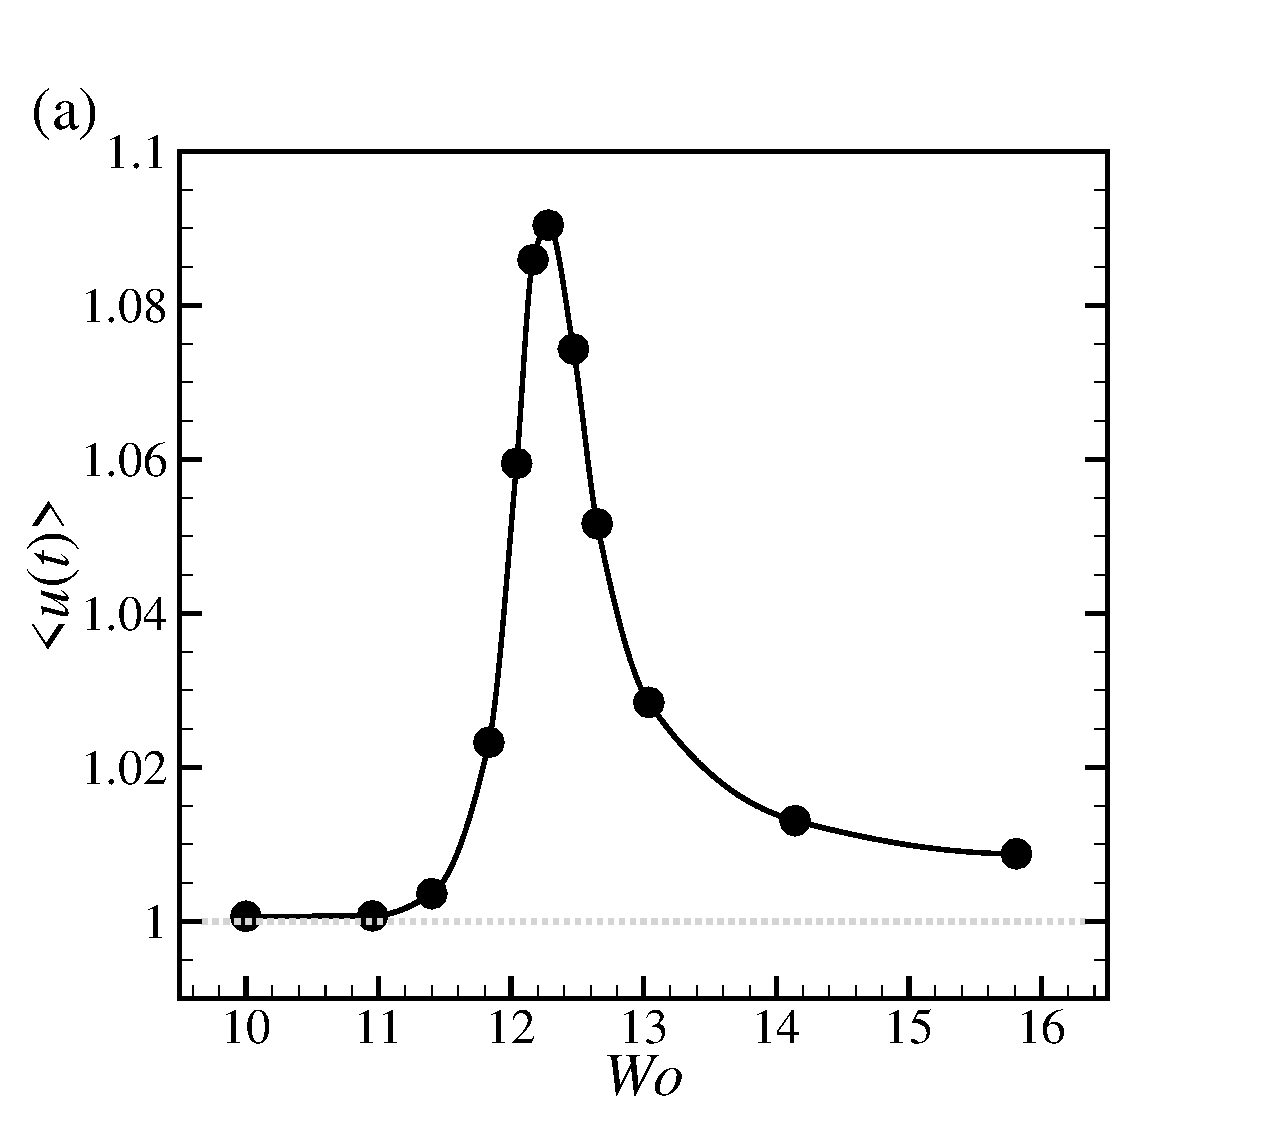
\includegraphics[width=0.49\linewidth, trim={0.2cm 0.4cm 0.4cm 0.5cm}, clip]{./epsFig/fig6a.eps}
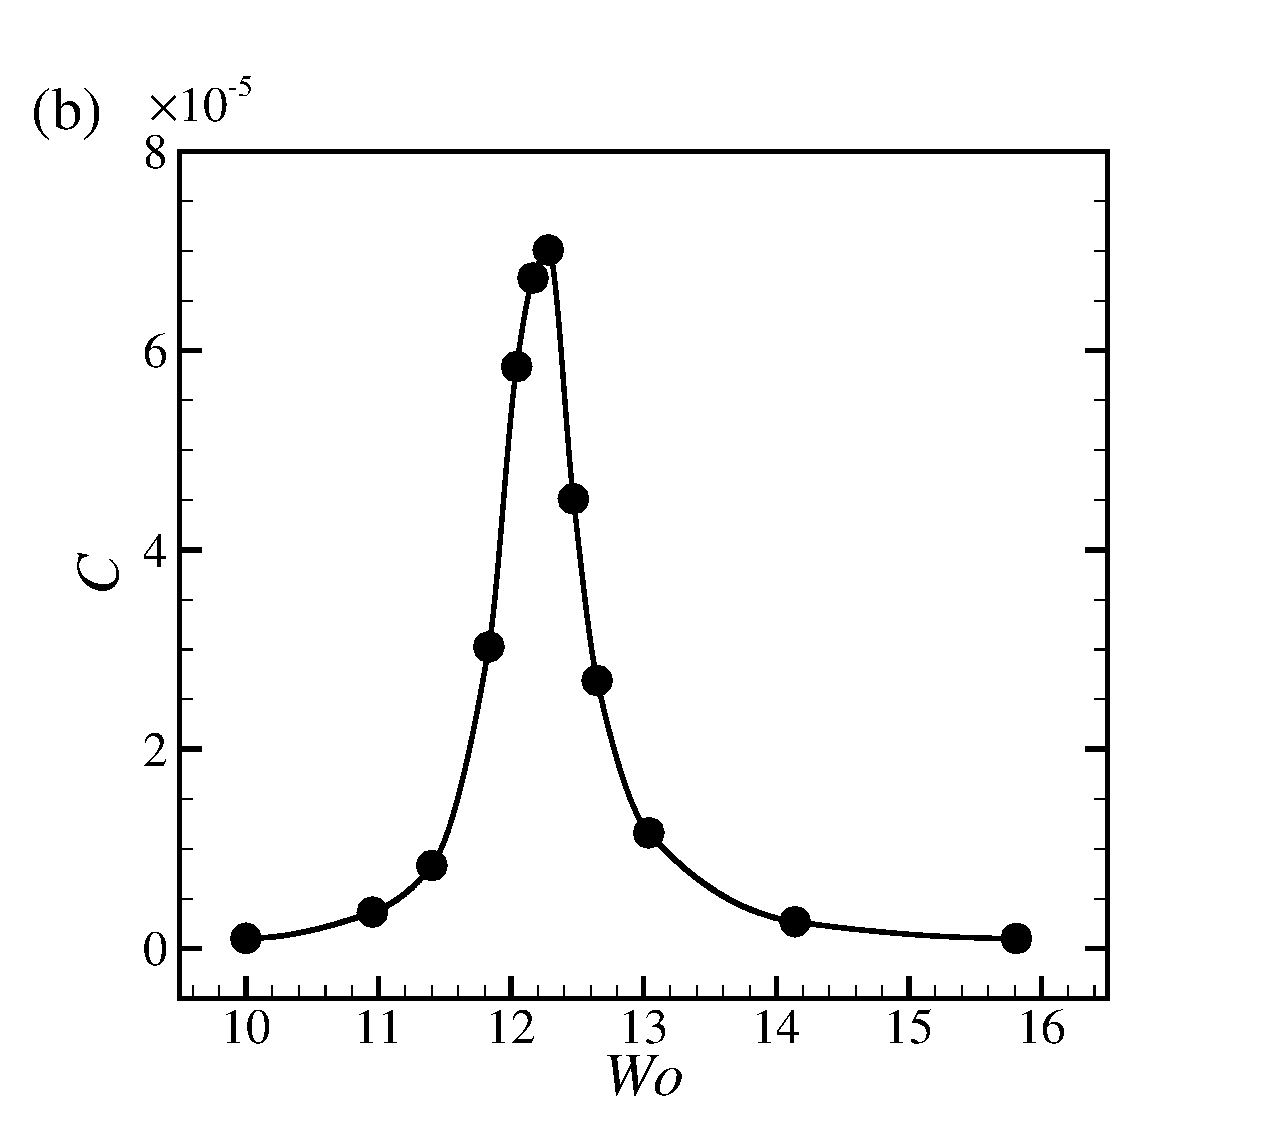
\includegraphics[width=0.49\linewidth, trim={0.2cm 0.4cm 0.4cm 0.5cm}, clip]{./epsFig/fig6b.eps}
\caption{(Color online) (a) Averaged streamwise fluid velocity $\langle u(t) \rangle$ against Womersley number $\Wo$ for $\Rey=100$, $Q=10^{-4}$ ($H=10^6$) and  $p_\mathrm{ext}=0.012$. (b) Flow compliance.}	\label{fig:flowrate_compliance}
\end{figure}
% Do not use Q for the flow rate (it may be confused with the other Q); actually this is the mean velocity
% Duo: changed.

The relationship between the driving pressure difference and the flow rate is important for fluid transport and has attracted much attention in studies of blood flows, where it is usually described with windkessel models \citep{Westerhof2009}.  %Citation is needed here % high citation paper
Figure~\ref{fig:flowrate_compliance}a shows the time-averaged streamwise velocity as a function of the Wommersly number. Here all other parameters were kept fixed, so that this figure illlustrates the effect of changing the pulsation frequency in a physical experiment. The external pressure was chosen such that the membrane oscillated with zero average deformation (i.e.\ about the height of the solid wall segments).  Interestingly, the mean velocity is higher than that of a rigid channel driven with a constant pressure difference, resulting in an enhancement of nearly 10\% close to the resonance point.
% More data is needed here; the resonance point should be marked. 
Similarly, the compliance $C$, obtained by the volume change of the channel over the corresponding pressure change (through a least-squared linear-fitting), features also a strong dependence on the frequency (see Fig.~\ref{fig:flowrate_compliance}b), a feature clearly not  present in windkessel models. %This suggests the necessity of accounting for a frequency-dependent compliance models for emphasizing local effects of the fluid-solid interaction \citep{vandeVosse11}. 


%%%%%%%%%%%%%%%%%%%%%%%%%%%%%%%%%%%%%%%%%%%%%%
% I have not touched the conclusions yet, we need to 
% a) discuss the implications for modeling collapsible flow vessels
% b) propose some experiments in a tube or channel to verify our theoretical predictions.
% c) We need to show how the effective exponent -1/6 shown in Figure 1b can be somehow predicted from the model (transient part of the solution, which I have deleted from this version), this should be quite easy.

In summary, we have shown that the dynamics of pulsatile flow in a channel with an elastic wall, which is a canonical model for blood flow in elastic vessels, exhibits complex dependencies on the material and flow parameters. Despite this complexity, the dynamics of the membrane can be entirely described with a simple harmonic oscillator model. 

\begin{acknowledgments}
D.X. gratefully acknowledges the support from Alexander von Humboldt Foundation (3.5-CHN/1154663STP).
\end{acknowledgments}

\bibliography{FSI}

\end{document}

